\setcounter{secnumdepth}{4}

\section{Introdução}

Linguagens de programação interpretadas têm sacrificado performance
em favor de um alto nível de abstração do funcionamento da máquina
envolvida, possibilitando maior expressividade, facilidade de
desenvolvimento, portabilidade, flexibilidade, dinamicidade, entre outras
características.
Especificamente, a linguagem de programação \texttt{Tcl}
(\textit{Tool Command Language}) teve como um de seus maiores
objetivos a facilidade de incorporação (\textit{embedding}) a
programas que desejassem ter uma linguagem de comandos
\cite{ousterhout_89}. Uma interface simples e extensível para
aplicações em linguagem \texttt{C} era o fator motivante de seu uso.
Programas inteiramente em \texttt{Tcl} eram vistos como pequenos
scripts, muitos talvez de uma linha no máximo \cite{ousterhout_89}.
Entretanto, aplicações em \texttt{Tcl} com milhares de linhas,
como por exemplo exmh \cite{exmh}, OpenACS \cite{openacs} ou mesmo a
suíte de testes do GDB (\textit{GNU Debugger}) \cite{gdb_testsuite},
tem surgido e a reescrita de trechos críticos em \texttt{C} vem sendo
aplicada para reduzir o impacto da máquina virtual no tempo de execução.

Outra forma de melhorar o desempenho de linguagens e, portanto,
reduzir a necessidade de reescrita de código em linguagens compiladas,
é por meio da utilização da compilação JIT (\textit{Just-In-Time}) que
realiza tradução de código sob demanda. No caso deste trabalho, estamos
interessados na tradução de \textit{bytecodes} da máquina virtual
\texttt{Tcl} para código de máquina durante o tempo de execução.
Informações acerca do programa em execução são coletadas
conforme necessário para guiar a compilação dinâmica. Portanto,
linguagens tipicamente difíceis de serem analisadas e compiladas
estaticamente, devido a uso de, por exemplo, tipagem dinâmica ou
escopo dinâmico, ganham a oportunidade de melhoria de desempenho
com uso de tal sistema de compilação.

O presente trabalho pretende melhorar o desempenho da linguagem
\texttt{Tcl}, reduzindo o tempo de decodificação e interpretação
de \textit{bytecodes} por meio da implementação e implantação de um
compilador JIT na mesma. Diversos trabalhos, como
\cite{deutsch84efficient} para a linguagem \texttt{Smalltalk},
Jalapeño \cite{jalapeno_1} para \texttt{Java}, Psyco \cite{psyco}
para \texttt{Python} ou a implementação do SELF-93 \cite{holzle},
demonstraram resultados bastante significativos ao implantar tal
método de compilação. Pretende-se ainda manter um nível de
manutenibilidade e flexibilidade adequado, permitindo extensões e
futuro desenvolvimento sobre este trabalho inicial.

Um compilador JIT requer que as estruturas internas sejam
suficientemente eficientes, caso contrário não se torna viável o
uso de um compilador otimizador em tempo de execução. As escolhas a
cerca de quais representações intermediárias utilizar, como estruturar
os dados, quais otimizações aplicar e algoritmos para diversas fases da
compilação, devem ser feitas de forma a conseguir balancear baixo
tempo de compilação com código gerado de alta qualidade. Ainda há o
quesito de consumo de memória principal, que, apesar da crescente
capacidade disponível, ainda costuma ser um recurso escasso em
dispositivos embarcados. Sabe-se que o interpretador \texttt{Tcl} está
presente em roteadores da Cisco, pois vem incluso no Cisco IOS
(\textit{Internetwork Operating Systems}), mas esse trabalho
não tem como foco tal tipo de dispositivo e, portanto, consumo de
memória não será um dos pontos levados em consideração. Porém, entre
os fatores complicadores consideramos também a manutenibilidade do
sistema. Um nível muito alto de abstração, como dito no início do
texto, impediria a utilização de um programa de desempenho crítico e,
por outro lado, um nível muito baixo dificultaria a correção/detecção de
problemas e melhorias gerais.
Uma alternativa para esse problema vem sendo desenvolvida no
projeto PyPy \cite{pypy}, onde um interpretador para uma linguagem
qualquer é escrito em \texttt{RPython} (uma implementação mais
restrita da linguagem \texttt{Python}) e o PyPy realiza a tradução do
mesmo para a
linguagem \texttt{C} incluindo (atualmente) juntamente um compilador
JIT. Entretanto, um
dos objetivos do trabalho discutido aqui é analisar como um sistema de
tamanho reduzido compete com sistemas mais robustos. Não se tem a
intenção de fornecer um ambiente de alto nível para construção de
outras máquinas virtuais com ou sem compiladores JIT para
\texttt{Tcl}, mas sim uma implementação específica e direta.
A escolha da
linguagem \texttt{C} reflete esse objetivo porque não adiciona novas
dependências ao núcleo da linguagem \texttt{Tcl} além de possibilitar
criação de programas com desempenho aceitável.

Procura-se visar a simplicidade, de forma que o trabalho desenvolvido
possa servir de base para expansão a novas arquiteturas e também para
aplicação de técnicas de compilação diversas sob a
\texttt{Tcl}. Na representação intermediária, quádruplas são
escolhidas para formar blocos básicos e
esses, por sua vez, são utilizados para definir grafos de fluxo de
controle que são diretamente utilizados na geração de código e também
podem servir de entrada a representação SSA
(\textit{Static Single Assignment}). A arquitetura IA-32 foi escolhida
como alvo, pois está presente em boa parte dos computadores de uso
pessoal, porém a linguagem \texttt{Tcl} atualmente executa em várias
outras arquiteturas. Nesse sentido, permitir portar para IA-64, ARM, e
outras, sem tornar a tarefa demasiadamente complicada faz parte da
simplicidade que se pretende obter.

A seção \ref{rev_biblio} realiza uma revisão bibliográfica relevando
trabalhos que, de alguma forma, buscaram melhorar a performance da
\texttt{Tcl}. Também descrevemos brevemente alguns projetos de
compiladores JIT que apresentam alguma semelhança com o nosso. Em
seguida, na seção \ref{proposta} é descrito uma proposta um pouco mais
detalhada a respeito desse compilador. Na seção \ref{desenvolvimento}
alguns detalhes do que já foi desenvolvido são apresentados, incluindo a
estrutura atual para quádruplas e blocos básicos, código de máquina
para IA-32, e também um pouco sobre a instalação e execução do
compilador JIT e do código nativo. As demais seções
se destinam a mencionar dificuldades encontradas até qui, além de
descrever o que será feito a partir do ponto em que se encontra o
trabalho.


\section{Revisão Bibliográfica}
\label{rev_biblio}

A linguagem \texttt{Tcl} já obteve ganhos de performance em diferentes
estudos feitos. Um deles, que atualmente faz parte da implementação da
linguagem, descrito em \citeonline{tcl_bytecode}, é a geração e a
interpretação de \textit{bytecodes}. Anterior a esse trabalho, foi
demonstrado em \citeonline{sah_tc} que o \textit{parsing} do código
realizado a todo momento para sua reinterpretação e também a conversão
excessiva entre tipos de dados, pois a \texttt{Tcl} trata tudo como
\textit{string},
eram os grandes consumidores do tempo de execução. Com esse trabalho
feito, a linguagem passou a utilizar representação dupla para os
valores presentes na execução do programa. Uma representação é
interna, possivelmente mais eficiente para se trabalhar. A outra é a
típica representação em \textit{string} que a linguagem sempre usou. Caso uma
delas não esteja disponível, a outra é utilizada para recriar essa
representação se necessário.

Um trabalho mais recente, descrito por \citeonline{vitale_catenation}, lida
com a eliminação do \textit{overhead} de decodificação dos
\textit{bytecodes}, introduzido pelo trabalho descrito anteriormente,
fazendo uso de \textit{templates} que contém as instruções em
código nativo utilizadas para interpretar cada \textit{bytecode}.
Esse código é obtido por meio da compilação do próprio interpretador
\texttt{Tcl} e cada \textit{template} é copiado múltiplas vezes,
numa área de memória alocada em tempo de execução, conforme a quantidade de
cada \textit{bytecode} gerado. Nesse mesmo trabalho, o interpretador foi
modificado de forma a sempre executar somente tal código formado por
uma concatenação de \textit{templates}, eliminando o \textit{overhead} de
decodificação. Demonstrou-se que em certos testes o desempenho da
linguagem pode melhorar em até 60\% com a aplicação dessa técnica.
Esse trabalho é provavelmente o mais próximo, quando considerando
somente a \texttt{Tcl}, do que se pretende produzir aqui.
Ele não gera código, mas cópia código já gerado por um compilador
estático e replica conforme necessário, fazendo os devidos
ajustes, em tempo de execução. Por um lado o tempo de ``compilação'' é
bastante baixo, porém, não dá espaço para técnicas de otimização e assim
limita o potencial de melhoria de desempenho.

Outros trabalhos, para diferentes linguagens, se assemelham mais com a
proposta aqui discutida. A busca por máquinas virtuais de alta
performance tem, atualmente, se dirigido principalmente a linguagem
\texttt{Java}. É comum a presença de compiladores JIT em máquinas
virtuais para essa linguagem, cada um com diferentes
características. A JUDO \cite{judo}, faz uso
de compilação dinâmica com dois tipos de compiladores e coleta
informações em tempo de execução. O primeiro desses compiladores é um
mais simples, que gera código rapidamente, destinado a compilação
de métodos invocados pela primeira vez. O segundo compilador é
utilizado quando informações coletadas indicam que certos métodos
são executados muito frequentemente e, portanto, estes podem se
beneficiar com a aplicação de otimizações. Essa recompilação dinâmica
é feita com o intuito de balancear o tempo gasto na compilação com o tempo
efetivamente gasto na execução do programa. Esse sistema trabalha com
a compilação de métodos por inteiro, assim como o trabalho proposto
aqui. Enquanto isso, o trabalho discutido em \citeonline{suganuma_pldi_2003}
avalia a aplicação de compilação dinâmica a regiões de código, evitando
a compilação de trechos raramente executados. Além disso, esse sistema
utiliza um modo misto de execução, na qual interpretação e execução de
código nativo se alternam. Nesse ponto, nosso trabalho e o de
\citeonline{suganuma_pldi_2003} se assemelham.

Nos dois trabalhos sobre JIT mencionados acima não há uma descrição
a cerca das representações intermediárias (IR) utilizadas. Porém, um
outro trabalho
apresentado sobre a JVM (\textit{Java Virtual Machine}) CACAO \cite{cacao},
descreve algo parecido com a nossa proposta. De forma semelhante com a
``TVM'' (\textit{Tcl Virtual Machine}), a JVM tem uma arquitetura de
pilha e a CACAO faz uma conversão para uma representação orientada a
registradores com uso de poucas instruções. O artigo por
\citeonline{suganuma_ibm} vai além, exibindo a evolução de uma JVM
desenvolvida na IBM onde, inicialmente, era utilizado uma IR baseado
em pilha, porém mais compacta que a representação em \textit{bytecodes} da
\texttt{Java}, e que mais tarde passou também a se basear em
registradores. Os autores argumentam que para conseguir balancear
performance e tempo foi necessário, além de outros avanços, fazer uso
de 3 representações: aquela que já existia (chamada de EBC --
\textit{Extended Bytecode}) e de mais duas baseadas em
registradores. Cada uma delas recebe um conjunto de otimizações, sendo
feito propagação e cópias de constantes, eliminação de código morto,
eliminação de verificação de exceção, e algumas outras, enquanto que na
forma de quádruplas. A última dessas aparece na forma SSA, com os nós
sendo formados por quádruplas.


\section{Proposta}
\label{proposta}

A seguir é discutido a proposta atual do projeto e sua evolução ao
longo da implementação.

Para chegar ao código de máquina final, esse projeto se propôs em
um primeiro momento estudar e definir qual subconjunto da linguagem poderia
se beneficiar mais com tal técnica. O subsistema de Entrada/Saída, por
exemplo, dificilmente ganharia em desempenho com compilação dinâmica
uma vez que o tempo gasto para transferência e aguardo por dispositivos
costuma ser muito maior que o tempo das outras operações envolvidas.
Por outro lado, operações aritméticas podem ser bastante favorecidas.
O trabalho feito no Psyco, mostra melhoria
de 109 vezes no tempo de execução para aritmética de inteiros e 10,9
vezes em aritmética de ponto flutuante \cite{psyco}. Após essa
primeira análise, vê-se que entre todos os
\textit{opcodes} definidos cerca de 100 deles são de
uso geral, enquanto que o restante é dedicado a alguns poucos comandos
pré-definidos. Além disso, por volta de 20 deles realizam a mesma
tarefa mas trabalham com operandos de tamanhos diferentes (1 ou 4
bytes). Também encontramos que dois \textit{opcodes} são obsoletos,
reduzindo um pouco mais o subconjunto de trabalho.

Em paralelo ao requisito acima, foi iniciado o projeto e
implementação de uma representação intermediária (IR) de nível
médio. Na versão anterior dessa proposta foi mencionado a existência
de uma IR de baixo nível, mas, baseado na experiência obtida durante a
implementação do gerador de código de máquina, concluiu-se que a
representação atual é melhor classificada como de nível médio
devido a distância da máquina alvo. Também num primeiro momento
sugerimos utilizar um conjunto reduzido de instruções (RISC), assim
como é feito na \textit{GNU lightning} \cite{gnu_lightning}, para
construir uma árvore de instruções mais próximas da máquina
alvo. Parte dessa decisão inicial ainda se mantém, o uso de algo
parecido com RISC, mas partimos para uso de quádruplas e sugerimos o
uso da representação SSA, que seria seguida dessa outra. Atualmente o
uso de SSA se enquadra em um trabalho futuro.
A escolha inicial por árvores foi devido
a existência de diversos métodos para seleção de
instruções que trabalham sobre essa forma de representação
\cite{ir_tree_parsing}, mas trabalhar com quádruplas se mostrou
simples.

O sistema de compilação dinâmica precisa ser
capaz de determinar quando iniciar e parar a geração de código.
Neste projeto atualmente é feito uso dos
limites de um procedimento como pontos de início e parada. Também é
interessante que o sistema colete informações, como de tipos
utilizados, para possivelmente permitir gerar código mais específico
para alguns trechos ou também analisar a forma com que certos procedimentos
são mais frequentemente utilizados. Alguns tipos numéricos da
\texttt{Tcl} vem sendo coletados durante a interpretação pela máquina
virtual mas ainda não são utilizados na compilação JIT.

Após essas etapas pretendia-se aplicar pelo menos algumas das
otimizações clássicas tais como remoção de código morto, propagação de
constantes e movimentação de código. A etapa de otimização foi
realocada para algum momento após a implementação do gerador de código
estar mais completo.

Chegamos, assim, na fase de seleção de instruções
seguida de alocação de registradores. Há diversos algoritmos, como
\textit{Maximal Munch}, seleção com uso de programação dinâmica ou
NOLTIS \cite{noltis}  para seleção de instruções além de vários
outros, por coloração de grafos ou mesmo por meio de uma varredura
linear \cite{linear_scan_regalloc} (com ou sem \cite{wimmer_franz}
desconstrução da representação SSA), para alocação de registradores.
Atualmente, a seleção de instruções é feita de forma
rudimentar (ou até mesmo inexistente). Cada quádrupla gerada define uma
instrução e esta, por sua vez, é utilizada durante a geração de código
para escolher um caminho no \textit{switch} de instruções e produzir
uma sequência de instruções de máquina pré-estabelecidas. Essa forma
de ``seleção'' é bastante econômica em termos computacionais, mas não
se preocupa com o custo combinado de instruções. % A alocação de
%registradores ... XXX ....
A possibilidade de métodos mais sofisticados ainda é
possível mas se tornou um ponto para um projeto futuro.

Finalmente temos a geração de código. O foco desse trabalho é a
arquitetura IA-32, que possui uma ampla quantidade de instruções, extensões e
diversas formas de endereçamento.
Porém, muitos dos recursos existentes não têm sido aproveitados de forma
forma a tornar factível a criação do gerador.
Idéias e trechos de trabalhos anteriores, como Harpy \cite{harpy}
ou o \textit{Tiny Code Generator} (incluído nas versões mais recentes do
QEMU \cite{qemu}), podem ser reutilizadas aqui mas até o momento a
implementação tem ocorrido seguindo manuais da Intel
\cite{intel_aam}\cite{intel_naz}. Ainda, de forma semelhante com a
etapa anterior, a infraestrutura permitirá a implantação de geração de
código para outras arquiteturas.


\section{Desenvolvimento}
\label{desenvolvimento}

A situação da implementação do compilador JIT até esse momento é descrita nas
subseções seguintes. Esta seção inicia detalhando como nosso
compilador foi introduzido na máquina virtual da linguagem \texttt{Tcl} e
também como é determinado os procedimentos a serem compilados. Em
seguida é descrito como pode ocorrer a execução do código de máquina
representado como uma sequência de bytes. A representação
intermediária e estruturas utilizadas são apresentadas na sequência e
são feitas considerações a respeito do projeto inicial. Finalmente
temos uma seção um pouco maior que descreve a geração de código
de máquina para a arquitetura IA-32 e uma breve consideração sobre
portabilidade para outras arquiteturas.


\subsection{Instalação e execução do compilador JIT}
\label{install-exec}
Para possibilitar a execução do compilador dinâmico em momentos
específicos durante a execução da própria máquina virtual alvo, algumas
modificações foram realizadas na implementação da
\texttt{Tcl}. Essas modificações efetivamente ``instalam'' o
compilador JIT no sistema original e serão descritas a seguir.

A linguagem \texttt{Tcl} invoca a função \verb!TclCreateProc! toda vez
que deseja associar a definição de um procedimento qualquer com uma
estrutura interna \verb!Proc!. Logo, a estrutura \verb!Proc! parece
ser um local ideal para ser aumentado pois todos procedimentos
criados, que foram escritos em linguagem \texttt{Tcl}, conterão uma
instância da mesma. Um campo com a estrutura de um
\verb!JIT_Proc! foi então inserido nessa outra estrutura.

\begin{figure}[h]
  \centering
  \begin{lstlisting}[language=C]
    struct JIT_Proc {
      int eligible;
      unsigned int callCount;
      unsigned char *ncode;
      int collectingTypes;
      struct JIT_BCType *bytecodeTypes;
    };
  \end{lstlisting}
  \caption{\label{jitproc}Estrutura que aumenta a Proc}
\end{figure}

Durante a execução da função \verb!TclCreateProc! a estrutura é apenas
inicializada. A manutenção dos campos dessa estrutura \verb!JIT_Proc!
depende de, em grande parte, chamadas a outra função,
\verb!TclObjInterpProcCore!. Essa,
por sua vez, é chamada por meio da \verb!TclObjInterpProc! que é associada
a um ponteiro \verb!Proc! por meio da função \verb!Tcl_ProcObjCmd! que
faz uso da função pública \verb!Tcl_CreateObjCommand!. A escolha da
\verb!TclObjInterpProcCore! foi, portanto, devido ao modo com que os
procedimentos escritos puramente em \texttt{Tcl} são criados
e executados internamente.
Portanto, a execução de um procedimento \texttt{Tcl},
criado da forma descrita anteriormente, necessariamente causa a
execução da função \verb!TclObjInterpProcCore!.

O campo \verb!collectingTypes!, inicializado em \verb!0!, é utilizado para
detectar se já foi alocado memória para o campo \verb!bytecodeTypes!
ou não, sendo atualizado para \verb!1! na primeira execução de uma
função escrita puramente em \texttt{Tcl}. O campo \verb!ncode! é
inicializado em \verb!NULL! e atualizado para um endereço quando for
gerado código de máquina para o procedimento. O campo \verb!callCount!
controla se o procedimento deve ir para compilação dinâmica ou não,
sendo decrementado a cada chamada e estabelecendo que o compilador JIT
deve ser invocado ao atingir
o valor \verb!0!. Atualmente esse campo é inicializado com o valor
\verb!1! (definido por \verb!JIT_REQINVOKE!),
indicando que o procedimento será interpretado uma vez antes
de ser possivelmente compilado para código de máquina e instalado em
seguida. O primeiro
campo, mas o último a ser descrito, é utilizado para definir se o
procedimento é elegível a compilação dinâmica ou não. A elegibilidade
é definida da seguinte maneira: se alguma execução do procedimento pelo
interpretador retornar um resultado que não seja \verb!TCL_OK!, então
o respectivo procedimento é marcado como não elegível. Isso é feito de
modo a tentar não gerar código que quase certamente terá que
tratar exceções.

Como foi dito, os campos da estrutura \verb!JIT_Proc! requerem
manutenção durante a execução da máquina virtual. Porém, o estado dessa
máquina pode mudar durante execuções subsequentes de um mesmo
procedimento. Para tratar o caso de mudanças, a \texttt{Tcl} sempre invoca a
função \verb!TclProcCompileProc! (a partir da \verb!TclObjInterProc!
rapidamente mencionada acima) antes de toda execução e verifica se o
procedimento já foi compilado para \textit{bytecode} e se houveram
mudanças em relação ao espaço de nomes (\textit{namespace})
relevante. Caso seja necessário, o procedimento é então recompilado,
ou compilado pela primeira vez, para \textit{bytecodes} e nesse ponto
também são reinicializados os campos da estrutura \verb!JIT_Proc!
correspondente.


\subsection{Execução do código de máquina}
\label{codeexec}
Uma parte da subseção anterior descreveu em que situação o código de
máquina para um procedimento específico é gerado e instalado. Agora será
apresentado como ocorre a execução do mesmo.

Tomando a estrutura \verb!JIT_Proc! da figura \ref{jitproc}
verifica-se a existência do campo \verb!ncode!, que é definido como
um ponteiro para \verb!unsigned char!. A indicação de que um
procedimento \texttt{Tcl} pode ter sua execução realizada por meio de
código de máquina direto ao invés de interpretação é a não nulidade do
\verb!ncode!. Tendo estabelecido um endereço para esse campo deve ser
possível requerer que tal endereço seja entendido como um endereço para
uma função. Se temos um endereço para uma função, devemos conseguir
invocar tal função passando os parâmetros esperados. A validade dessas
duas últimas tarefas se deve ao fato de que uma função qualquer é
simplesmente uma sequência de bytes que foi gerada por algum
compilador para alguma arquitetura. Porém, realizar essas tarefas pode
requerer uma certa flexibilidade da linguagem que se deseja
utilizar. No caso da linguagem \texttt{C}, que foi a escolhida para
esse projeto, é permitido realizar um \textit{cast} adequado que
resolve esse problema. Especificamente, queremos tratar o endereço em
\verb!ncode! como um ponteiro para uma função que recebe dois
parâmetros e que tem como resultado um valor inteiro;
em seguida invocamos passando os dois parâmetros:
\verb!((int (*)(void *, void *))ncode)(param1, param2)!. A escolha
dessa assinatura é devido àquela existente para a função
\verb!TclExecuteByteCode!. Essa última função mencionada é invocada
por meio da \verb!TclObjInterpProcCore! nos casos em que o compilador
JIT não gerou código de máquina para um procedimento. Manter a
compatibilidade entre essas duas funções, passando os mesmo
parâmetros, proporciona ao código gerado pelo compilador JIT tratar
objetos literais, parâmetros do procedimento \texttt{Tcl}, variáveis
locais e outros detalhes de forma bastante similar ao da
implementação da \verb!TclExecuteByteCode!.


\subsection{Representação Intermediária}
A seguir é apresentado a evolução das escolhas feitas a respeito da
representação intermediária para o compilador discutido e também o
estado atual da mesma.

Inicialmente a proposta descrevia o uso de uma forma de representação
intermediária em árvore. A intenção era, em uma etapa mais adiante,
fazer uso de um algoritmo, entre os diversos existentes, para seleção
de instruções que se baseiam em árvores. % Junto com esse fato,
%observa-se que o uso de otimizações durante a geração de código não
%havia sido explicitado no texto anterior.
Porém, a partir da leitura de
textos diversos essa decisão inicial foi repensada de forma a
simplificar ainda mais o projeto.
Sendo assim, a etapa de especificação do compilador JIT
definiu o uso de uma representação intermediária linear inicial de nível
médio na forma de
quádruplas. Ainda estava previsto a transformação para a forma SSA que
tem sido considerada por diversos compiladores, como LLVM
\cite{llvm1}, GCC \cite{gcc-ssa} e Jalapeño (ou Jikes RVM)
\cite{jalapeno_1}. Tal representação foi deixada para um projeto futuro,
mas vale ressaltar que um dos principais motivos para uso da SSA, de
acordo com \citeonline{cytron}, é a possibilidade de executar certas
otimizações clássicas de maneira eficiente
enquanto nessa IR, destacando eliminação de redundância parcial,
propagação de constante e movimentação de código.
A construção do grafo de fluxo de controle (CFG
-- \textit{Control Flow Graph}) de um trecho de código específico faz
parte dos requisitos para a transformação em SSA, porém ele também é
atualmente utilizado diretamente na geração de código pelo compilador
desse trabalho. Com isso
chegamos a outra decisão: o uso de quádruplas para compor blocos
básicos que representam os nós do CFG.

A representação em quádruplas é relativamente simples de se construir,
além de apresentar uma característica relevante para a otimização que
realiza movimentação de código: mover uma quádrupla tende a requerer
menor esforço do do que rearranjar uma representação em forma de
árvore. Entretanto, conforme discutido em \citeonline[p. 96]{muchnick},
também é possível que a representação em árvore apresente vantagens
em relação à utilizada, sendo a eliminação de registradores virtuais
temporários e armazenamentos nos mesmos uma delas.

Na versão atual do compilador a estrutura apresentada na figura
\ref{quad-struct} representa uma quádrupla.

\begin{figure}[h]
  \centering
  \begin{lstlisting}[language=C]
    struct Quadruple {
      Value *dest;
      unsigned char instruction;
      Value *src_a, *src_b;
      struct Quadruple *next;
    };
  \end{lstlisting}
  \caption{Estrutura para uma quádrupla\label{quad-struct}}
\end{figure}

O campo \verb!instruction! tem tipo \verb!unsigned char! pois atualmente
representa um dos \textit{bytecodes} da \texttt{Tcl} ou uma das
instruções \verb!JIT_INST_MOVE!, \verb!JIT_INST_CALL!,\\
\verb!JIT_INST_GOTO!, \verb!JIT_INST_JTRUE!, \verb!JIT_INST_JFALSE!,
\verb!JIT_INST_ADD!,\\ \verb!JIT_INST_INCR!, que podem ser representadas com um
byte -- todas elas tem um número associado no intervalo [0, 255].
O campo \verb!next! existe para
lidar de forma eficiente com casos de otimização que requerem a
movimentação de código, apesar de otimizações ainda não terem sido
implementadas. Também temos os campos de tipo \verb!Value! que,
inicialmente, permitia assumir valores inteiros, ponteiros para
\verb!Tcl_Obj! ou uma forma de registrador. Na versão atual essa
estrutura foi aumentada com os campos \verb!flags! e \verb!offset!. O
primeiro desses é utilizado para indicar onde o valor deverá
ser encontrado em tempo de execução. O outro descreve um deslocamento
para o valor caso o mesmo se encontre em um \textit{array}.

Para agrupar as quádruplas e formar os blocos básicos apresentamos a
estrutura seguinte:

\begin{figure}[h]
  \centering
  \begin{lstlisting}[language=C]
    struct BasicBlock {
      int id;
      int exitcount;
      struct Quadruple *quads, *lastquad;
      int *exitblocks;
    };
  \end{lstlisting}
  \caption{Estrutura para um bloco básico}
\end{figure}

Como não há um campo ``\verb!next!'' nessa abstração, guardamos o
número de arcos, em \verb!exitcount!, que saem de um bloco de modo a
permitir o controle de sua travessia por meio do campo
\verb!exitblocks!. O ponteiro \verb!lastquad! é
utilizado na construção do CFG, eliminando a necessidade de travessia das
quádruplas presentes em um bloco para identificar se a última
instrução é de desvio ou não. O campo \verb!id! serve, até o momento,
somente para \textit{debugging}. A identificação dos blocos básicos e
construção do CFG não difere daquela apresentada em
\citeonline[p. 173-175]{muchnick}, porém não é feito, até o momento, o
uso de blocos básicos estendidos. A visualização dos blocos básicos
ainda não ocorre de forma didática, sendo possível apenas uma exibição
em modo texto bastante simples; com algum esforço é possível
transformar essa saída em uma entrada para algum programa que trata do
desenho de grafos.
% Em breve
%espera-se gerar código na linguagem \texttt{dot} ou fazer uso do
%aplicativo xfig para facilitar essa tarefa. Ainda assim é possivel
%analisar o que é gerado e, para isso, tomamos o código exemplo seguinte:
 %Para visualizar os blocos básicos, e tornar
%mais fácil a verificação, foi criada uma função que escreve na
%linguagem \texttt{dot} o conteúdo contido nessas estruturas. Dado um
%código como:

Para exemplificar um CFG construído, consideremos o procedimento
descrito na figura \ref{fig:gray}.
\begin{figure}[h]
  \centering
  \begin{lstlisting}[language=Tcl]
    proc grayb {n} {
      for {set i 0} {$i < 2 ** $n} {incr i} {
        puts [expr {$i ^ ($i >> 1)}]
      }
    }
  \end{lstlisting}
  \caption{Procedimento que exibe código Gray de números com até n
    bits \label{fig:gray}}
\end{figure}
Feita uma pequena modificação na implementação é possível definir
\verb!JIT_REQINVOKE! em 0 e, antes da primeira execução interpretada do
código, conseguimos exibir o CFG. Ao executar ``\verb!grayb 2!''
teremos que a função \verb!JIT_Compile! (nome segue o padrão de
nomenclatura do código fonte da \texttt{Tcl} para funções públicas)
será chamada pela função
\verb!TclObjInterpProcCore!, essa última foi modificada conforme
descrito na subseção \ref{install-exec}. Após a execução da
\verb!JIT_Compile! temos como um dos resultados o grafo de fluxo de
controle, que para o código acima será aquele exibido na figura \ref{bbs}.
%Essa última é invocada pela própria
%\texttt{Tcl} e fica responsável por chamar a função que realiza a
%interpretação de \textit{bytecodes}, a
%\verb!TclExecuteByteCode!. Pretende-se realizar a coleta de tipos
%durate a execução dessa última função mencionada, alterando-a de
%acordo com as necessidades do compilador JIT. Enfim, ao término
%da função \verb!JIT_Compile! o grafo de fluxo de controle exibido a
%seguir é obtido.

\begin{figure}[h]
  \centering
  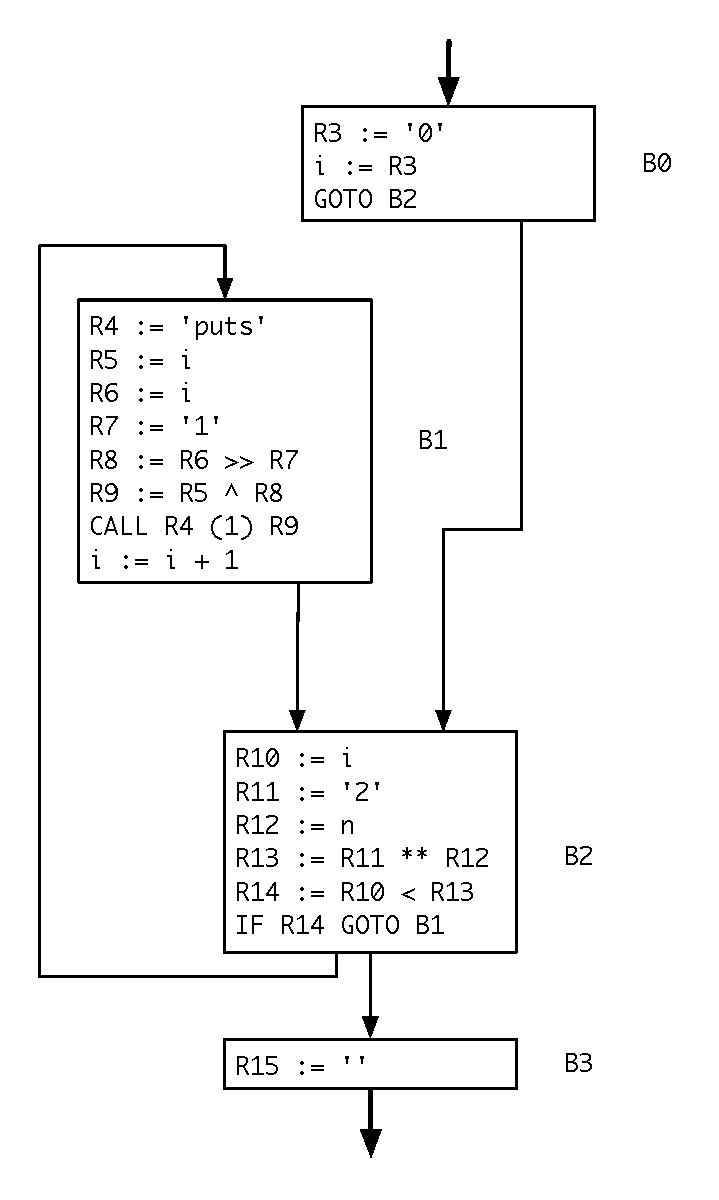
\includegraphics[scale=0.68]{bbs}
  \caption{Blocos básicos e grafo de fluxo de controle construídos \label{bbs}}
\end{figure}

Para se chegar nessa representação foi feita uma espécie de conversão de
máquina virtual baseada em pilha para algo se assemelha
com uma máquina de infinitos registradores. Uma pilha temporária é
utilizada para simplificar essa transição, sendo acessada e atualizada
durante a construção de diversas instruções. Também são pré-alocados
registradores virtuais para as variáveis locais. A implementação da
\texttt{Tcl} disponibiliza uma lista dinâmica com todas essas
variáveis locais, incluindo também os parâmetros formais da função,
sendo necessário apenas atribuir índices a elas. O registrador
\verb!R1! está associado ao parâmetro \verb!n!, mas nunca é acessado
diretamente porque o programa exemplo não altera seu valor. Por outro
lado, o \verb!R2! que associa-se a variável local \verb!i! é utilizado
mas foi renomeado (de \verb!R2! para \verb!i!) na figura \ref{bbs} para
deixar mais claro seu uso.

Verifica-se que há diversas instruções de atribuição que recebem um
valor que se parecem com números, como \verb!'0'! ou \verb!'1'!, mas
que estão sendo representados como \textit{strings}. Na realidade esses valores
são todos ponteiros para uma estrutura \verb!Tcl_Obj!, podendo assumir
qualquer tipo interno presente na linguagem. Nesse exemplo podemos
assumir, e de fato assim ocorrerá, que todos são inteiros. No caso da
\textit{string} \verb!'puts'! armazenada no registrador 4 tem-se que ela
servirá como chave em uma tabela \textit{hash} que possui como valor a
respectiva função (ou não, gerando um erro). Todos esses ponteiros
estarão armazenados num \textit{array} quando a função for executada,
sendo necessário definir os campos \verb!flags! e \verb!offset! da
estrutura \verb!Value! correspondente de acordo.
O número entre parênteses na instrução \verb!CALL!
indica que haverá 1 parâmetro na chamada e, no caso, este será o
conteúdo de \verb!R9!. A única instrução no bloco de saída B3 indica o
valor de retorno de função -- uma \textit{string} vazia.

Haviam 55 \textit{bytecodes} (não exibidos aqui) sendo utilizados para
representar o código da figura \ref{fig:gray}, e agora 18 quádruplas
são empregadas com o mesmo resultado. Nessa quantidade numérica
superior destaca-se o uso de 9 bytes para representar a instrução
\verb!INST_START_CMD! da \texttt{Tcl}, destinando 1 byte para o código
da instrução em si, 4 bytes para indicar a posição relativa do início
do próximo comando e
4 bytes para contar a quantidade de comandos que fazem parte desse que
está iniciando de modo a possibilitar ao  interpretador respeitar
limites impostos para certos recursos por meio de
APIs específicas. Porém, apesar das quádruplas estarem em número inferior,
levando em conta o total de bytes contidos em cada quádrupla (de
acordo com as estruturas acima) tem-se que
o consumo de memória é bastante superior mas temporário -- após
a geração de código as quádruplas não precisam mais estar em memória.
Ao mesmo tempo é possível observar que muitas delas são passíveis a
eliminação, ficando a cargo de otimizações em etapas futuras.

Um último esclarecimento a respeito da figura \ref{bbs} precisa ser feito.
Os \textit{bytecodes} de desvio emitidos pela \texttt{Tcl} utilizam
operandos que descrevem posições relativas (negativas ou positivas) à
posição atual mas pode-se notar que na
representação utilizada há somente desvios absolutos para blocos
básicos. Para essa tarefa foi feito um mapeamento de cada
\textit{bytecode} para cada bloco básico antes de construir o
conteúdo dos blocos assumindo que não haveriam mais quádruplas do que
\textit{bytecodes}.

\subsubsection{Mapeamento de alguns \textit{bytecodes} para quádruplas}

A seguir é realizada uma breve análise de como alguns
\textit{bytecodes} são convertidos para quádruplas e, em um caso
específico, verifica-se um indício de possível erro durante execução
de código que poderia ter sido gerado pelo compilador JIT.

Na figura \ref{fig:gray} não foi feito uso de variáveis globais, então
começaremos analisando a saída gerada para um trecho que faz uso de
tal recurso. O exemplo da figura \ref{fig:global1} é bastante simples,
porém incorreto na linguagem \texttt{Tcl}. É necessário preceder
explicitamente a variável de seu escopo, no caso o escopo global é
simbolizado por ``\verb!::!''. Também é possível utilizar o comando
\verb!global! para indicar uma lista de variáveis como globais.

\begin{figure}[h]
  \centering
%  \begin{lstlisting}[language=Tcl, numbers=left]
  \begin{lstlisting}[language=Tcl]
    set x 4
    proc y {} { puts $x }
    y
  \end{lstlisting}
  \caption{Uso incorreto de variável global em
    \texttt{Tcl} \label{fig:global1}}
\label{xx$xx}
\end{figure}

Ao executar tal código o interpretador gera uma exceção, mas, antes de
exibir a descrição do problema, a função \verb!JIT_Compile! é
chamada (assumindo que \verb!JIT_REQINVOKE! ainda está definida em \verb!0!).
O resultado, ajustado para melhor visualização, é exibido na
tabela \ref{tabela1}.

\begin{table}[h]
  \centering
  \caption{Saída produzida para procedimento da figura \ref{fig:global1} \label{tabela1}}
  \begin{tabular}{| p{4cm} | p{4cm} |}
    \hline
    \bf{Bytecode} & \bf{Registradores} \\
\begin{verbatim}
PUSH 'puts'
LOAD_SCALAR x
INVOKESTK 2
DONE
\end{verbatim} &
\begin{verbatim}
R2 := 'puts'
R3 := 0x0
CALL R2 (1) R3
\end{verbatim} \\
    \hline
  \end{tabular}
\end{table}

Os registradores 2 e 3 estão sendo atribuídos a endereços de memória
estruturados como \verb!Tcl_Obj!. Por esse motivo, fica claro que não
há um endereço previsto para a variável \verb!x! e, portanto, esse
código certamente geraria um erro (assim como o interpretador gera em
seguida) se fosse compilado para código de máquina.%  Corrigindo,
% alterando para imprimir \verb!$::x!, a seguinte sequência de bytecodes
% e de registradores é produzida:

% \begin{table}[h]
%   \centering
%   \caption{Saída produzida para procedimento corrigido da figura 5}
%   \begin{tabular}{| p{4cm} | p{4cm} |}
%     \hline
%     \bf{Bytecode} & \bf{Registradores} \\
% \begin{verbatim}
% PUSH 'puts'
% PUTS '::x'
% LOAD_SCALAR_STK
% INVOKESTK 2
% DONE
% \end{verbatim} &
% \begin{verbatim}
% R1 := 'puts'
% R2 := '::x'
% ...
% CALL R1 (1) R2
% \end{verbatim} \\
%     \hline
%   \end{tabular}
% \end{table}

%%% NEXT_INST_V(1, 1, 1)

Continuando ainda no exemplo da figura \ref{fig:global1}, detalhamos
como o mapeamento de uma coluna para outra foi realizado no restante
dessa seção. Começando
pela instrução \verb!DONE! vemos que
nada equivalente aparece na coluna a direita. Isso é resultado da
atual simplificação feita na outra representação, que, diferentemente
da máquina virtual em execução, não verifica por exceções e tão pouco
por código de retorno anormal -- tais tarefas são realizadas em
diversos trechos da função \verb!TclExecuteByteCode! mas também são
especificamente feitas na execução da instrução \verb!DONE!.

A instrução \verb!PUSH! é mapeada fazendo uso de uma pilha temporária e
também de um \textit{array} de objetos literais. Um operando que segue a
instrução \verb!PUSH! é tomado como o índice nesse \textit{array}, sendo
possível obter o objeto esperado. O registrador criado nesse momento,
\verb!R2! no exemplo, é
inserido no topo da pilha temporária. A instrução \verb!LOAD_SCALAR!
é mapeada de forma similar, mas ela se baseia em obter o
endereço da variável escalar de uma lista de variáveis locais
criada pelo compilador da \texttt{Tcl} para o procedimento
corrente. Nesse momento temos os registradores 2 e 3 nessa pilha e
então a instrução \verb!INVOKESTK! deve ser convertida. Seguida de um
operando, chamado de \verb!objc! aqui, indicando a quantidade total de
argumentos -- incluindo o nome da função -- temos que os elementos
$0 \dots objc - 2$ da pilha a partir do topo são os parâmetros para
a função na posição $objc - 1$ a partir do topo. Na representação
utilizada não é contado o nome da função como um parâmetro, por isso
entre parênteses vê-se o número 1 ao invés do 2.


\subsection{Geração de código de máquina}
\label{codegen}
Sabendo como a representação intermediária é formada e como o sistema
trabalha para executar o código gerado, falta ainda descrever como tal
código de máquina é gerado.

Logo após a criação do CFG, a função \verb!JIT_CodeGen! é invocada e o
seu resultado é um ponteiro para \verb!unsigned char! que em seguida é
passado para um campo \verb!ncode! de um procedimento específico. A
função \verb!JIT_CodeGen! faz todo o trabalho que cabe a
esta seção.

\subsubsection{Reservando e controlando espaço para os bytes}
A primeira questão a ser tratada é onde colocar os bytes que serão
gerados. De acordo com a seção \ref{codeexec}, uma função é apenas uma
sequência de bytes que pode ser executada. De forma direta poderíamos
pensar em deixar os bytes em um região de memória alocada por
uma função como a \verb!malloc!. Simplesmente fazer isso não garante
que o sistema permitirá a execução dessa sequência de bytes.

Com a introdução do bit NX (\textit{No-eXecute}) pela AMD e depois
pela Intel (que renomeou para \textit{eXecute-Disable}), o hardware
passou a poder prevenir a execução de código em páginas destinadas a
dados \cite[seção 5.13]{intel_prog} e, dessa forma, elimina
parcialmente ataques relacionados a \textit{buffer
  overflow}\footnote{O artigo ``Code Injection Attacks on
  Harvard-Architecture Devices'' de Aurélien Francillon e Claude
  Castelluccia publicado na ACM CCS 2008 menciona trabalhos que
  contornam a proteção por bit NX além de outras proteções que
  tem sido desenvolvidas.}.
Por essa razão uma região de
memória alocada por meio do \verb!malloc! não poderá ter seu conteúdo
executado em sistemas que fazem uso desse recurso. Uma forma de
corrigir esse problema é fazer uso da função \verb!mprotect!,
definindo a região com proteção de leitura e execução após escrever os dados
desejados. Entretanto, essa função requer que o tamanho da região
alocada seja um múltiplo do tamanho de página -- denominado de
\textit{page-aligned}. Para resolver este outro problema faz-se uso da função
\verb!memalign! ou \verb!valloc! de acordo com a disponibilidade. Porém, nota-se que
o mais adequado é definir o tamanho da região como um múltiplo do
tamanho de página, eliminando a necessidade de alinhamento e reduzindo
questões de portabilidade. A quantidade de bytes que define o tamanho
de uma página pode ser obtido com a função
\verb!getpagesize!. A estrutura exibida na figura \ref{mcode-struct}
juntamente com as funções \verb!pagesize!, \verb!newpage! e
\verb!pagenowrite! exibidas no apêndice A
tratam dos problemas mencionados de forma similar a descrita e também
de questões de portabilidade entre Windows e UNIX.

\begin{figure}[h]
  \centering
  \begin{lstlisting}[language=C]
    struct MCode {
      unsigned char *mcode, *codeEnd;
      int limit, used;
    };
  \end{lstlisting}
  \caption{Estrutura para controlar uso de memória do código sendo gerado\label{mcode-struct}}
\end{figure}

Os campos \verb!limit! e \verb!used! determinam o tamanho total
alocado e o espaço usado até o momento, respectivamente. Atingindo o
valor limite, uma nova página precisa ser alocada e o campo
\verb!limit! tem seu valor dobrado. Os campos \verb!mcode! e
\verb!codeEnd! apontam para o início do código de máquina e o
ponto atual na região de memória, respectivamente. O endereço contido em
\verb!mcode! é aquele que será instalado no campo
\verb!ncode! da estrutura \verb!JIT_Proc! de um procedimento
específico caso a geração de código tenha sucesso.

\subsubsection{Código de máquina IA-32}

A arquitetura IA-32 tem sido amplamente utilizada nos computadores de
uso pessoal, mantendo portabilidade a nível de código objeto desde o
processador 8086 e fazendo uso de um conjunto de instruções complexo (CISC).
Essa última característica reflete a grande quantidade de instruções
existentes nessa arquitetura (e que tem aumentando) e também a
variedade de combinações permitidas. Convenções a cerca de chamadas de
funções também tem sido estabelecidas, formando parte de uma interface
binária de aplicação (ABI). Nesse trabalho seguiu-se a ABI para
chamada de funções descrita em \citeonline{systemv-abi}, que é a mesma
seguida pelo Linux e quase a mesma pelo Mac OS X (ver \citeonline{macosx-abi}).

%\paragraph{Modos de endereçamento}
%\quad \\
% XXX

\paragraph{Início e término da geração}
\quad \\
Antes de gerar código específico para um CFG, a função
\verb!JIT_CodeGen! gera um prólogo genérico que pode ser visto na
figura \ref{prologo-epilogo}. Após toda a geração do código novamente
temos um código genérico, agora chamado de epílogo e que também é
apresentado na figura \ref{prologo-epilogo}. A divisão da pilha em
partes (\textit{frames}) origina o conceito de \textit{stack frame}
que é manuseado pelo código do prólogo. Cada \textit{stack frame} pode
variar de tamanho, e por isso definimos um ponto base para acessar
parâmetros ou variáveis locais de forma que seja respeitada as
condições da ABI. Essa base, ou ponto de referência, fica definida como
o endereço contido no registrador \verb!ebp! após a execução do
prólogo. É possível encontrar definições de prólogo que incluam código
para salvar os registradores \verb!ebx!, \verb!edi!, \verb!esi!
e \verb!esp! uma vez que, de acordo com a ABI seguida, esses
registradores (além do \verb!ebp! que já é salvo) precisam ser
preservados entre chamadas. Na
implementação atual, código para salvar qualquer um desses
registradores precisa ser gerado conforme necessário. O epílogo possui
código antônimo daquele contido no prólogo, efetivamente desfazendo o
\textit{stack frame} construído e retornando para o endereço contido
na topo da pilha corrente.

\begin{figure}[h]
  \centering
  \begin{lstlisting}[language=C, numbers=left]
#define PROLOGUE(code)   \
    PUSH_REG(code, EBP); \
    MOV_REG_REG(code, ESP, EBP)
#define EPILOGUE(code) LEAVE(code); RETN(code)

#define PUSH_REG(code, reg) *code++ = 0x50 + reg
#define MOV_REG_REG(code, src, dest) \
    *code++ = 0x89;                  \
    *code++ = MODRM(0x3, src, dest)
#define LEAVE(code) *code++ = 0xC9
#define RETN(code) *code++ = 0xC3

#define MODRM(mod, reg, rm) (mod << 6) + (reg << 3) + rm
  \end{lstlisting}
  \caption{Código para epílogo e prólogo breve em x86\label{prologo-epilogo}}
\end{figure}

Assume-se que \verb!code! seja um ponteiro da forma do \verb!codeEnd!
da estrutura \verb!MCode! (figura \ref{mcode-struct}) e disponha de
uma região de memória suficiente para a execução correta dessas macros.

Na figura \ref{prologo-epilogo}, entre as linhas 1 a 4 têm-se algo
semelhante com código em \texttt{Assembly} de sintaxe
AT\&T. A partir da linha 6 observa-se um trabalho semelhante, porém
simplificado, de um montador para x86. Para entender o significado das
linhas 6, 8, 9 e 13 apresenta-se a tabela \ref{mov-push-1} com formato
similar àquelas encontradas nos  manuais da Intel
\cite{intel_aam}\cite{intel_naz} mas
adaptada para sintaxe AT\&T e reduzida para as necessidades da situação.

\begin{table}
  \caption{Uma variação das instruções MOV e PUSH\label{mov-push-1}}
  \centering
  \begin{tabular}{l l l l c}
    \toprule
    Opcode  & Instrução     & Operando 1    & Operando 2    &  Modo 64-Bits \\
    \midrule
    0x89 /r & \verb!MOV r32, r/m32!& ModRM:reg (r) & ModRM:r/m (w) &  Válido       \\
    0x50+rd & \verb!PUSH r32!      & reg (r)       &               &  N.C.         \\
    \bottomrule
  \end{tabular}
\end{table}

Na coluna ``\textit{Opcode}'' da tabela \ref{mov-push-1} encontram-se
os códigos hexadecimais das variações de \verb!MOV! e \verb!PUSH!
utilizadas e também as informações ``/r'' e ``+rd''. A primeira dessas
indica que a instrução faz uso de um byte chamado de ModR/M que segue
o valor hexadecimal. Esse byte ModR/M é divido em três partes: mod (2 bits),
reg/opcode (3 bits) e r/m (3 bits), da direita para esquerda seguindo
a ordem \textit{little-endian}. O byte final é formado conforme
a linha 13 da figura \ref{prologo-epilogo}.
A parte ``reg/opcode'' determina ou um
número de registrador ou mais três bits de informação de acordo com
a especificação do \textit{opcode} (que não é utilizado aqui). O campo
``r/m'' ou específica um registrador como um operando ou pode ser
combinado com o ``mod'' para codificar um modo de endereçamento. Para
mais detalhes sobre o byte ModR/M recomenda-se a consulta ao manual da
\citeonline[capítulo 2]{intel_aam}. Retomando à coluna
``\textit{Opcode}'', a informação ``+rd'' indica que um código entre 0
e 7, simbolizando um registrador de 32 bits, deve ser somado ao valor
em hexadecimal. A segunda coluna da mesma tabela indica que os operandos são
registradores de 32 bits (\verb!r32!) ou que pode-se buscar algum
conteúdo no endereço de memória calculado (\verb!r/m32!). No
caso dessa variação do \verb!MOV! queremos mover dados de um
registrador para outro. A última coluna da tabela indica se o
\textit{opcode} apresentado pode ser utilizado no modo 64-bits ou não;
no caso desse \verb!PUSH! está sendo indicado que a sintaxe da instrução
não é codificável no modo 64-bits. Ou seja, essa última coluna
consegue indicar quais das instruções atualmente codificadas pelo
compilador teriam que ser no mínimo ajustadas para que pudéssemos
trabalhar com a arquitetura x64.

%+rd indica um registrador por meio de um código entre 0 e 7. A letra
%``d'' vem de ``dword'' (contração de ``doubleword'')
%e implica no uso de registradores de 32 bits.

%/r sinaliza que o byte ModR/M da instrução contém um operando
%na forma de registrador e um operando r/m
As colunas da tabela \ref{mov-push-1} relacionadas aos operandos são
discutidas agora. Encontra-se entre parênteses ``r'' ou ``w'',
significando que o conteúdo do operando será ou lido
(\textit{\textbf{r}ead}) ou atualizado
(\textit{\textbf{w}ritten}) pelo processador. O único operando dessa
instrução \verb!PUSH! é um registrador, indicado por ``reg''. Para a
instrução \verb!MOV! utilizada, dispomos de 32 combinações de
endereçamento devido ao uso do byte ModR/M. Entretanto, estamos
interessados apenas na especificação de registradores. De acordo com a
tabela 2.2 do manual em \citeonline[seção 2.1.5]{intel_aam} verifica-se
que é necessário estabelecer o campo ``mod'' do byte ModR/M em 3 para
essa situação e, assim, juntamente com os números dos registradores fonte e
destino conseguimos completar esse byte adicional. Dessa forma, a
linha 9 do código da figura \ref{prologo-epilogo} está resolvida.


\paragraph{Percorrendo blocos e gerando código}
\quad \\
Uma busca em profundidade é disparada partindo do nó (bloco básico) na posição
0 do CFG e a cada bloco visitado ocorre geração de código para aquele
bloco. Uma quádrupla por vez do bloco básico corrente é acessada e um
\textit{switch} de instruções define qual cláusula corresponde a
instrução contida na quádrupla. Determinada a instrução que deverá ter
código gerado, chegamos ao assunto principal dessa subseção.

Devido a granularidade alta, imposta pela representação intermediária
atual, mesmo uma instrução simples como a \verb!JIT_INST_INCR! requer uma
quantidade relativamente alta de bytes para codificá-la e, portanto,
podemos aproveitá-la para uma discussão detalhada.

\begin{figure}[h]
  \centering
  \begin{lstlisting}[language=Tcl]
    proc myinc {x} {
      return [incr x]
    }
  \end{lstlisting}
  \caption{Código exemplo para análise da instrução JIT\_INST\_INCR \label{myinc}}
\end{figure}

O exemplo da figura \ref{myinc} gera apenas um bloco básico com
apenas uma quádrupla. O comando \verb!incr! da \texttt{Tcl} permite
que uma variável, que pode ter seu valor representado como um inteiro,
seja incrementada ou decrementada em qualquer quantidade inteira.
Porém, o compilador
JIT, ao detectar o bytecode \verb!INST_INCR_SCALAR1_IMM! (criado pela
\texttt{Tcl} para o comando \verb!incr!) codifica-o
como \verb!JIT_INST_INCR! somente se o valor absoluto do incremento
for 1. Para os demais casos uma instrução \verb!JIT_INST_ADD! é estabelecida.
Nesse exemplo temos o comportamento padrão do comando \verb!incr!, que
incrementa em 1 unidade a variável indicada. Feitas essas
considerações partimos efetivamente para o código de máquina, um pouco
simplificado, desse trecho.

Assumindo que a instrução \verb!JIT_INST_INCR! tenha sido corretamente
codificada, o valor do operando A (campo \verb!src_a! da estrutura
\verb!Quadruple! -- figura \ref{quad-struct}) necessariamente contém uma
indicação de que o operando é uma variável local. Sendo assim,
precisamos chegar a essa variável local. Na seção \ref{codeexec} foi
descrito a assinatura da função criada pelo compilador JIT mas ainda
não foi dito quais os tipos dos parâmetros que seriam
passados. Seguindo a compatibilidade com a função
\verb!TclExecuteByteCode!, o primeiro parâmetro é uma estrutura
interna denominada \verb!Interp! que será utilizada para chegar a
variável local. Tendo essa informação, os primeiros bytes a serem
gerados aqui dizem respeito a movimentação do primeiro parâmetro para
um registrador.
\begin{figure}[h]
  \centering
  \begin{lstlisting}[language=C]
#define COPY_PARAM_REG(code, paramn, reg) \
    MOV_DISP8DREG_REG(code, 8 + 4 * paramn, EBP, reg)

#define MOV_DISP8DREG_REG(code, disp, src, dest) \
    *code++ = 0x8B;                              \
    *code++ = MODRM(0x1, dest, src);             \
    *code++ = disp
  \end{lstlisting}
  \caption{Cópia de parâmetro para registrador seguindo ABI escolhida\label{copy-param}}
\end{figure}
O código na figura \ref{copy-param} realiza essa
função de acordo com a ABI escolhida. Assumindo um uso da forma:
\verb!COPY_PARAM_REG(code, 0, EAX)!, teremos em tempo de execução o
endereço de uma estrutura \verb!Interp! no registrador
\verb!eax!. Note que aqui temos outra variação da instrução
\verb!MOV!, que pode ser traduzida para \textit{assembly} como:
\verb!movl 8(%ebp), %eax!. Nesse ponto podemos atravessar a estrutura até
chegarmos ao \textit{array} que contém todas as variáveis locais --
trecho de código na figura \ref{goto-varstruct}.

\begin{figure}[h]
  \centering
  \begin{lstlisting}[language=C]
    long int offset;
    offset = offsetof(Interp, varFramePtr);
    MOV_DISP8DREG_REG(code, offset, EAX, EAX);
    offset = offsetof(CallFrame, compiledLocals);
    MOV_DISP8DREG_REG(code, offset, EAX, EAX);
  \end{lstlisting}
  \caption{Percorrendo Interp até variáveis locais\label{goto-varstruct}}
\end{figure}

Na estrutura \verb!Interp! tem-se que o campo \verb!varFramePtr!
aponta para um \verb!CallFrame! que possui acesso as variáveis atualmente em
uso. A estrutura \verb!CallFrame!, por sua vez, tem um
\verb!array! de tipo \verb!Var!, chamado de \verb!compiledLocals! e
que guarda as variáveis locais. Portanto, a figura
\ref{goto-varstruct} gera código equivalente a:
\verb!interp->varFramePtr->compiledLocals!, assumindo
que \verb!interp! aponte para o parâmetro de tipo
\verb!Interp!. Prosseguindo, faz-se uso do campo
\verb!offset! da estrutura \verb!Value! de \verb!src_a!, deslocando em
\verb!compiledLocals! até o ponto desejado e tornando possível acessar
o \verb!Tcl_Obj! que representa a variável local procurada -- ver figura
\ref{goto-localvar}, continuação da figura \ref{goto-varstruct}. Note
que a variável que queremos acessar aqui é um parâmetro para a função
escrita em \texttt{Tcl} e, além disso, é o primeiro parâmetro e, por
essa razão, o deslocamento será 0 no \verb!array! \verb!compiledLocals!.

\begin{figure}[h]
  \centering
  \begin{lstlisting}[language=C]
#define ADD_IMM8_REG(code, imm, reg) \
    *code++ = 0x83;                  \
    *code++ = MODRM(0x3, 0, reg);    \
    *code++ = imm


    if (src_a->offset) {
      ADD_IMM8_REG(code, sizeof(Var) * src_a->offset, EAX);
    }
    offset = offsetof(Var, value.objPtr);
    MOV_DISP8DREG_REG(code, offset, EAX, EAX);
  \end{lstlisting}
  \caption{Acessando variável local\label{goto-localvar}}
\end{figure}

Estando sobre o objeto desejado, é possível obter o valor inteiro
contido no mesmo (se houver). Entretanto, o endereço desse objeto será
reutilizado antes do código de máquina terminar e, portanto, salva-se
em outro registrador (se possível). O código na
figura \ref{inc-tclobj} avança até o ponto em que o valor contido no
objeto é incrementado, simplificações são feitas de modo que é
assumido que o objeto já construiu uma representação de tipo inteiro.

\begin{figure}[h]
  \centering
  \begin{lstlisting}[language=C]
#define INC_DREG(code, reg)      \
    *code++ = 0xFF;              \
    *code++ = MODRM(0x0, 0, reg)


    MOV_REG_REG(code, EAX, EDX);

    offset = offsetof(Tcl_Obj, internalRep.longValue);
    ADD_IMM8_REG(code, offset, EAX);
    INC_DREG(code, EAX);
  \end{lstlisting}
  \caption{Salvando endereço e incrementando em uma unidade uma variável local\label{inc-tclobj}}
\end{figure}

Nesse momento a variável local já foi incrementada mas ainda
precisamos realizar algumas tarefas antes de retornar. De acordo com o
funcionamento da \texttt{Tcl}, é
necessário definir o objeto resultado da função \verb!myinc! para o
interpretador em que a função executa. A linguagem
\texttt{Tcl} faz uso da função \verb!Tcl_SetObjResult! para tal
operação. Também é necessário atualizar a representação em
\verb!string! do objeto incrementado. Depois dessas tarefas podemos
retornar o código \verb!TCL_OK! (\verb!0!) para indicar sucesso.
O código contido nas figuras \ref{myinc-last-macros} e \ref{myinc-last}
realiza essas tarefas finais.

\begin{figure}[ht!]
  \centering
  \begin{lstlisting}[language=C]
#define PUSH_DISP8REG(code, disp, reg) \
    *code++ = 0xFF;                    \
    *code++ = MODRM(0x1, 6, reg);      \
    *code++ = disp
#define MOV_IMM32_REG(code, imm32, reg) \
    *code++ = 0xB8 + dest;              \
    IMM32(code, imm32)
#define CALL_ABSOLUTE_REG(code, reg) \
    *code++ = 0xFF;                  \
    *code++ = MODRM(0x3, 2, reg)
#define POP_REG(code, reg) *code++ = 0x58 + reg
#define XOR_REG_REG(code, src, dest) \
    *code++ = 0x33;                  \
    *code++ = MODRM(0x3, src, dest)

#define IMM32(code, v) \
    *code++ = v; *code++ = v >> 8; \
    *code++ = v >> 16; *code++ = v >> 24
  \end{lstlisting}
  \caption{Macros adicionais requeridos pela figura \ref{myinc-last}\label{myinc-last-macros}}
\end{figure}

\begin{figure}[ht!]
  \centering
  \begin{lstlisting}[language=C]
    /* Chamar Tcl_SetObjResult. */
    PUSH_REG(code, EDX);
    PUSH_DISP8REG(code, 8, EBP);
    MOV_IMM32_REG(code, (ptrdiff_T)Tcl_SetObjResult, ECX);
    CALL_ABSOLUTE_REG(code, ECX);

    /* ``Remove'' 8(%ebp) da pilha. */
    ADD_IMM8_REG(code, 4, ESP);

    /* Atualizar representacao string por meio da
     * funcao updateStringProc do tipo do objeto. */
    POP_REG(code, EDX);
    MOV_REG_REG(code, EDX, ECX);
    offset = offsetof(Tcl_Obj, typePtr);
    MOV_DISP8DREG_REG(code, offset, ECX, ECX);
    offset = offsetof(Tcl_ObjType, updateStringProc);
    MOV_DISP8DREG_REG(code, offset, ECX, ECX);
    PUSH_REG(code, EDX);
    CALL_ABSOLUTE_REG(code, ECX);

    ADD_IMM8_REG(code, 4, ESP);

    /* Retornar TCL_OK (ver ABI). */
    XOR_REG_REG(code, EAX, EAX);
  \end{lstlisting}
  \caption{Tarefas finais para o código da figura \ref{myinc}\label{myinc-last}}
\end{figure}

Após concluir a geração de código para a quádrupla atual, verifica-se
que não há mais quádruplas ou mesmo outros blocos a serem visitados. A função
\verb!JIT_CodeGen! está pronta para encerrar; ajustando a permissão
das páginas utilizadas e retornando
o endereço inicial para essa sequência de bytes que pode ser executada
como uma função. Para a figura \ref{myinc} foram utilizados 51 bytes,
o código de máquina para esse trecho é dado por:
\begin{verbatim}
0x8B 0x45 0x08 0x8B 0x40 0x64 0x8B 0x40 0x28 0x8B 0x40 0x04 0x89
0xC2 0x83 0xC0 0x10 0xFF 0x00 0x52 0xFF 0x75 0x08 0xB9 0x66 0x02
0x09 0x0A 0xFF 0xD1 0x83 0xC4 0x04 0x5A 0x89 0xD1 0x8B 0x49 0x0C
0x8B 0x49 0x0C 0x52 0xFF 0xD1 0x83 0xC4 0x04 0x33 0xC0 0xC3
\end{verbatim}

%Com esse código gerado funcionando podemos descrever como eliminar a
%suposição de que o objeto a ser incrementado contém um valor inteiro
%coerente na união \verb!internalRep! (ver figura \ref{inc-tclobj}).
% XXX Se continuar aqui vou precisar detalhar labels
% pendentes.. talvez essa seção fique demasiadamente longa.

Apesar do bytecode codificado acima ser um dos mais simples, é
possível reutilizar boa parte desse código para alguns outros. Uma
instrução de adição ou subtração entre uma variável e uma constante
qualquer requer somente a troca da \verb!INC_DREG! por uma outra
similar a já exibida \verb!ADD_IMM8_REG!. A parte do código que acessa
variáveis locais também pode ser reaproveitada por grande parte das
demais instruções \texttt{Tcl}. Além disso, serve de base para remoção
de pelo menos uma simplificação: a falta de verificação por
\textit{overflow}. Após incrementar a variável, poderíamos fazer uso
de um desvio condicional baseado na \textit{flag} \verb!OF!, do
registrador \verb!EFLAGS! (ver \citeonline[seção 3.4.3]{intel_basicarch}),
para um ponto de retorno que indica que
ouve \textit{overflow}. O compilador JIT, quando completo, precisa no
mínimo fazer esse tratamento e reiniciar a execução do procedimento por meio
de interpretação em vista que a linguagem \texttt{Tcl}
trabalha com números inteiros de tamanho arbitrário de forma
transparente.

Nesta seção foi considerado que detalhar todos os formatos das instruções aqui
codificadas seria uma distração. O leitor é convidado a visitar as
tabelas \ref{instr-encoding} e \ref{op-encoding} no apêndice A que
descreve todas as instruções codificadas nesse documento juntamente
com os nomes das macros utilizadas.


\subsubsection{Infraestrutura}

Até o momento já foram apresentadas diversas macros que efetivamente
geram código de máquina para a arquitetura IA-32. Agora é rapidamente
discutido como o gerador de código encontra estas definições.

O gerador de código encontra as definições adequadas a serem
utilizadas a partir de um arquivo de cabeçalho
(\verb!generic/jit/arch/arch.h! no código fonte) que faz a seleção
baseado em definições do compilador utilizado. No caso desse trabalho,
a linguagem \texttt{Tcl} tem sido compilada exclusivamente com o
\texttt{gcc} e a existência da definição \verb!__i386__! foi
suficiente para inclusão das macros esperadas. Portar o gerador para
outra arquitetura implica em: ajuste desse arquivo que faz a seleção do
que incluir e, também, a adaptação das macros existentes para esse outro
conjunto de instruções.

%\subsubsection{Limitações (ou Simplificações?)}
%XXX
%


\section{Dificuldades Encontradas}

A primeira dificuldade encontrada foi em relação a aprendizagem
(parcial) do funcionamento da linguagem de programação \texttt{Tcl} --
especificamente a versão 8.5.8 --
que contém mais de 200 mil linhas de código \texttt{C}. Boa parte
desse número de linhas não afeta diretamente a construção desse
compilador, porém uma grande quantidade será ativada
ao longo da execução do código gerado pelo compilador.

A linguagem faz uso de contagem de referências para realizar coleta de
lixo e também compartilha muitos dos valores utilizados. Com isso,
reutilizar objetos \verb!Tcl_Obj! (atualmente no caso da função
\verb!JIT_Compile!) que foram construídos em partes distintas não é tão
simples pois é necessário se ter certeza de que o objeto não será
desalocado enquanto se está trabalhando com ele e, ao mesmo tempo, não
se quer deixar objetos com contagem de referência superior a
necessária. Compartilhar objetos economiza memória mas não simplifica
o uso de objetos alheios, sendo necessário verificar se um objeto
específico é compartilhado ou não antes de, dependendo do uso,
duplicar o mesmo. Não são tarefas tão complexas mas tendem a ser
pontos de erros obscuros em programas não tão curtos e não tão simples.

Com o avanço da implementação, descrita nesse relatório, a geração de
código nativo realizada de forma manual demonstrou-se bastante
propensa a erros. Detalhes na geração do byte ModR/M causaram muitas
falhas de segmentação até chegar ao código final correto; saídas
produzidas pelo compilador gcc, analisada pelas ferramentas \verb!otool! ou
\verb!objdump!, ajudaram na correção ao longo do processo.

\section{Próximos Passos}

Devido ao tempo restante espera-se que somente duas atividades
continuem sendo desenvolvidas:
\begin{enumerate}
\item Geração de código para uma maior quantidade de bytecodes
  \texttt{Tcl} de modo a possibilitar análise coerente de resultados;
\item Escrita do texto final.
\end{enumerate}

\section{Conclusões}

Compiladores JIT tem sido implementados em máquinas virtuais que demandam
alta performance. Entre as linguagens de programação, \texttt{Java} se
destaca ao ter recebido suficiente atenção ao ponto de empresas e
pesquisadores desenvolverem diversas JVMs com compiladores
dinâmicos que fazem uso de uma variedade de técnicas.

Escolhas adequadas para todas as partes de um compilador JIT tornam
possível o uso de um compilador otimizador em tempo de execução. Esse
texto teve maior foco nas representações intermediárias utilizadas, ou
que se pretende utilizar, nesse projeto. Quádruplas para formar blocos
básicos e permitir a construção do grafo de fluxo de controle (CFG)
foi mais discutida aqui, mas também foi mencionado a representação SSA
que inicia-se com a entrada de um CFG. A SSA tem sido aplicada em
diversos compiladores otimizadores, pois permite aplicar, ao menos,
as otimizações de movimentação de código, propagação de constante e
eliminação de redundância parcial de forma eficiente.

A conversão de \textit{bytecodes} de uma máquina de pilha para uma
representação na forma de máquina de registradores exige atenção aos
detalhes da semântica implementada na máquina virtual atual da
linguagem. Uma vantagem visível é a capacidade de sintetização que
uma representação baseada em registradores tem sobre uma que faz uso
de pilha. Entretanto, um número reduzido de quádruplas não indica
necessariamente menor consumo de memória do que uma quantidade
superior de \textit{bytecodes}.

Detalhes relacionados a definição de onde instalar o compilador JIT na
linguagem alvo e de quando executar a compilação JIT envolvem pelo
menos um entendimento simplificado do funcionamento da máquina
virtual. Com a experiência adquirida até o momento, essa etapa aparenta
ser a mais simples de ser feita.

A geração de código de máquina, em especial para uma arquitetura CISC,
de forma manual é dispendiosa e propensa a erros. Apesar da alta
granularidade imposta pela representação intermediária atual,
mostrou-se necessidade de 51 bytes para a codificação simplificada de um
procedimento em \texttt{Tcl} com um único comando
\verb!incr!. Entretanto, discute-se que, entre essa quantidade total,
um número significativo de bytes pode ser reaproveitado por muitas das
outras instruções para acesso a variáveis locais. Além disso, com
pequenas alterações é possível codificar outras instruções simples, ou
variações do \verb!incr! que não façam uso de incremento de valor
absoluto 1, da linguagem \texttt{Tcl}.

% XXX mais ?


% Referências
\bibliography{biblio}


%\newpage

\section*{Apêndice A}

\renewcommand\lstlistingname{Código}

\begin{lstlisting}[language=C, caption={Alocação de página(s) para o
    compilador JIT}, frame=tb]
void *
newpage(void *size)
{
    void *page;
#ifdef _WIN32
    page = VirtualAlloc(NULL, *((DWORD *)size),
                        MEM_COMMIT | MEM_RESERVE,
                        PAGE_EXECUTE_READWRITE);
    if (!page) {
        perror("VirtualAlloc");
        exit(1);
    }
#else
    page = mmap(NULL, *((size_t *)size),
                PROT_READ | PROT_WRITE | PROT_EXEC,
                MAP_ANON | MAP_PRIVATE, 0, 0);
    if (page == MAP_FAILED) {
        perror("mmap");
        exit(1);
    }
#endif
    return page;
}
\end{lstlisting}


\begin{lstlisting}[language=C, caption={Tamanho, em bytes, de uma
    página}, frame=tb]
#ifdef _WIN32
DWORD
pagesize(void)
{
    DWORD pagesize;
    SYSTEM_INFO si;
    GetSystemInfo(&si);
    return si.dwPageSize;
}
#else
int pagesize(void)
{
    return getpagesize();
}
#endif
\end{lstlisting}


\begin{lstlisting}[language=C, caption={Remoção da permissão de
    escrita de uma ou mais páginas}, frame=tb]
void
pagenowrite(void *page, size_t len)
{
#ifdef _WIN32
    DWORD oldProtect;
    if (VirtualProtect(page, len, PAGE_EXECUTE_READ,
                       &oldProtect) == 0) {
        perror("VirtualProtect");
        exit(1);
    }
#else
    if (mprotect(page, len, PROT_READ | PROT_EXEC) < 0) {
        perror("mprotect");
        exit(1);
    }
#endif
}
\end{lstlisting}

\newpage

\renewcommand{\arraystretch}{1.2}

\begin{table}[ht!]
  \caption{Variações das instruções codificadas, sintaxe AT\&T\label{instr-encoding}}
  \centering
  \begin{tabular}{l l c l}
    \toprule
    Opcode  & Instrução     & Cod. Oper.    & Macro \\
    \midrule

    0x83 /0 ib & \verb!ADD imm8,r/m32! & A  & \verb!ADD_IMM8_REG! \\

    0xFF /2 & \verb!CALL r/m32! & B & \verb!CALL_ABSOLUTE_REG! \\

    0xFF /0 & \verb!INC r/m32! & C & \verb!INC_DREG! \\

    0x89 /r & \verb!MOV r32,r/m32!& D & \verb!MOV_REG_REG! \\
    \hline
    0xB8+rd & \verb!MOV imm32,r32! & E & \verb!MOV_IMM32_REG! \\
    & & & \verb!MOV_DISP8DREG_REG! \\
    \hline

    0x58+rd & \verb!POP r32!     & F & \verb!POP_REG!\\

    0x50+rd & \verb!PUSH r32!    & G & \verb!PUSH_REG!\\
    0xFF /6 & \verb!PUSH r/m32!  & B & \verb!PUSH_DISP8REG!\\

    0x33 /r & \verb!XOR r32,r/m32!& A & \verb!XOR_REG_REG! \\

    \bottomrule
  \end{tabular}
\end{table}

\begin{table}[ht!]
  \caption{Codificações para os operandos da tabela \ref{instr-encoding}\label{op-encoding}}
  \centering
  \begin{tabular}{c l l}
    \toprule
    Cod. Oper. & Operando 1 & Operando 2 \\
    \midrule
    A & imm8 & ModRM:r/m (r,w) \\
    B & ModRM:r/m (r) & \\
    C & ModRM:r/m (r,w) & \\
    D & ModRM:reg (r)& ModRM:r/m (w) \\
    E & imm32 & reg (w) \\
    F & reg (w) & \\
    G & reg (r) & \\
    \bottomrule
  \end{tabular}
\end{table}
